\section{Đặc trưng âm học của tiếng nói}
\subsection{Mô hình bộ máy phát âm:}
Trong mô hình bộ máy phát âm, hệ thống phát âm của con người được xem như một bộ máy tạo ra các tín hiệu âm thanh 
thông qua sự kết hợp của các thành phần chính: nguồn âm thanh (nguồn rung động từ dây thanh), bộ lọc 
(hệ thống cộng hưởng của khoang miệng, mũi và họng), và bức xạ (sự phát tán âm thanh ra môi trường bên ngoài). 
Nguồn âm thanh tạo ra sóng âm cơ bản, sau đó được điều chỉnh và biến đổi bởi bộ lọc để tạo ra các đặc trưng âm học 
khác nhau.\\
\begin{figure}[ht]
  \centering
  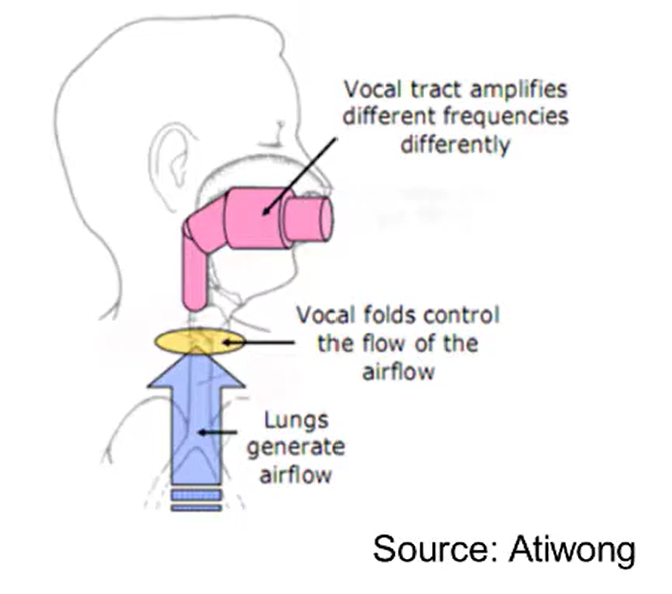
\includegraphics[width=0.5\textwidth]{./graphics/Dac_trung_am_hoc_0.png} % PNG/JPG/PDF
  \caption{Mô hình bộ máy phát âm}
  \label{Mô hình bộ máy phát âm}
\end{figure}\\
Bức xạ từ bộ lọc ra môi trường bên ngoài có 2 thành phần chính:
\begin{itemize}
    \item Tần số cơ bản (fundamental frequency - F0): là tần số dao động cơ bản của dao động dây thanh,
    tạo ra âm thanh có cao độ (pitch) nhất định. Xấp xỉ 110Hz, 200Hz, 400Hz tương ứng với các giọng nam, nữ và trẻ em.
    \item Các tần số cộng hưởng formants (F1, F2, F3, ...): là các tần số đặc trưng được tạo ra bởi hệ thống cộng hưởng của bộ lọc khoàng miệng, mũi và họng, là thứ quyết định âm sắc. 
    Các tần số này thường có tần số cao hơn với tần số cơ bản F0 và đóng vai trò quan trọng trong việc xác định đặc trưng âm học của các nguyên âm khác nhau.
\end{itemize}
Trong phát âm, chúng ta thường có 2 loại âm thanh chính:
\\
\begin{figure}[ht]
  \centering
  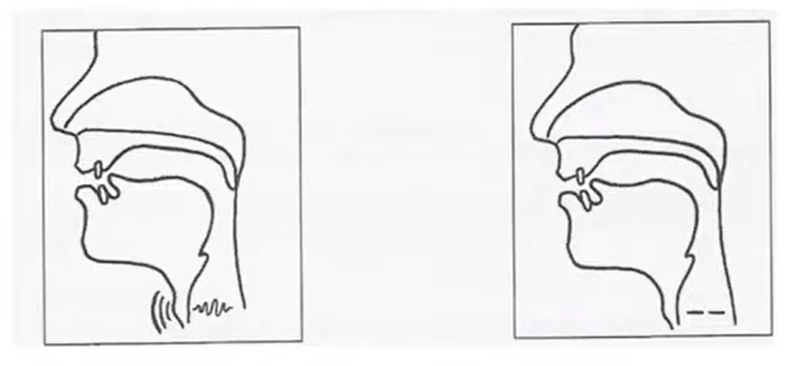
\includegraphics[width=0.5\textwidth]{./graphics/Dac_trung_am_hoc_1.png} % PNG/JPG/PDF
  \caption{Âm vô thanh và âm hữu thanh}
  \label{Âm vô thanh và âm hữu thanh}
\end{figure}\\
\begin{itemize}
    \item Khi phát âm các âm hữu thanh (voiced sounds), dây thanh rung động, tạo ra nguồn dao động có tần số F0.
    \item Khi phát âm các âm vô thanh (unvoiced sounds), dây thanh mở hoàn toàn, không rung động, nguồn 
    dao động chủ yếu là tiếng ồn (noise) được tạo ra từ luồng khí đi qua các hẹp trong khoang miệng do đó các âm này thường 
    có tần số cơ bản F0 thấp, chủ yếu phân bố âm thanh ở tần số cao. Thường được mô phỏng giống nhiễu.
\end{itemize}
Một số ví dụ về các âm sắc khác nhau:
\begin{table}[!htp]
\centering
\caption{Ví dụ về các âm sắc khác nhau}
\begin{tabular}{|l|p{4cm}|p{6cm}|}
\hline
\textbf{Trường hợp} & \textbf{Mô tả âm sắc} & \textbf{Đặc trưng phổ (liên quan đến MFCC)} \\ \hline
Âm /a/ (mở rộng miệng) & Âm sáng, vang, cộng hưởng mạnh ở tần số thấp (~700 Hz) & Formant F1 cao, F2 trung bình \\ \hline
Âm /i/ (miệng hẹp) & Âm sáng, có năng lượng ở tần số cao hơn & F1 thấp, F2 cao \\ \hline
Âm /u/ (tròn môi) & Âm tối, ấm & F1 thấp, F2 thấp \\ \hline
Âm /s/ (xì) & Âm sắc gắt, nhiều năng lượng cao tần & Năng lượng tập trung ở 4-–8 kHz \\ \hline
Âm /f/ (sh) & Âm sắc “mềm” hơn /s/, năng lượng thấp hơn & Phổ nghiêng về 2--4 kHz \\ \hline
Âm /z/ (hữu thanh của /s/) & Giống /s/ nhưng có năng lượng nền ở thấp tần do dây thanh rung & Thêm dải năng lượng thấp (~100–300 Hz) \\ \hline
Nam nói /a/ vs Nữ nói /a/ & Giọng nam ấm, trầm hơn; giọng nữ sáng hơn & Formant tương tự, nhưng F\textsubscript{0} và độ lệch phổ khác \\ \hline
Đàn guitar vs Violin (nốt La) & Khác nhau ở cấu trúc hài (overtones) & Phổ của violin có hài cao mạnh hơn, âm sắc sáng hơn \\ \hline
Âm /p/ (phụ âm vô thanh bật hơi) & Âm sắc sắc, năng lượng ngắn ở cao tần & Burst noise ngắn ở phổ cao \\ \hline
Âm /b/ (phụ âm hữu thanh tương ứng) & Âm mềm hơn, có năng lượng ở thấp tần & Thêm năng lượng do rung dây thanh \\ \hline
\end{tabular}
\end{table}
\newpage
\subsection{Phân tích MFCC}
Như chúng ta đã phân tích ở phần trước, các đặc trưng âm học của tiếng nói chủ yếu được quyết định bởi tần số cơ bản F0 và các tần số cộng hưởng formants. 
Do đó, để khai thác các đặc trưng này, chúng ta tập trung vào việc phân tích phổ tần số của tín hiệu âm thanh.
\subsubsection{Biến đổi FFT:}
Biến đổi Fourier nhanh (\textbf{Fast Fourier Transform} -- FFT) là một thuật toán hiệu quả để tính \textit{Biến đổi Fourier rời rạc} (DFT) của một dãy tín hiệu số.  
Nếu ta có một tín hiệu rời rạc $x[n]$ gồm $N$ mẫu, khi đó DFT của tín hiệu này được định nghĩa như sau:

\[
X[k] = \sum_{n=0}^{N-1} x[n] \, e^{-j \frac{2\pi}{N} kn}, \quad k = 0, 1, 2, \ldots, N-1
\]

Trong đó:
\begin{itemize}
    \item $x[n]$ là tín hiệu trong miền thời gian.
    \item $X[k]$ là phổ tần số tương ứng tại chỉ số $k$.
    \item $N$ là số mẫu của tín hiệu.
    \item $j$ là đơn vị ảo, với $j^2 = -1$.
\end{itemize}

Thuật toán FFT giúp giảm đáng kể độ phức tạp tính toán của DFT từ $O(N^2)$ xuống còn $O(N \log N)$ bằng cách khai thác tính chất đối xứng và tuần hoàn của các hệ số mũ phức trong công thức DFT.\\

\textbf{Ý nghĩa:} Kết quả của FFT, $X[k]$, biểu diễn biên độ và pha của các thành phần tần số có trong tín hiệu $x[n]$. 
Giải thuật này cho phép chúng ta phân tích chuỗi tín hiệu trong miền tần số.\\
\subsubsection{Biến đổi Fourier ngắn hạn (Short-Time Fourier Transform - STFT)}
Nhằm tránh mất mát thông tin, một file âm 
thanh dài sẽ được chia nhỏ thành các frame có chồng lấp, sau đó ta áp dụng FFT và hàm 
windowing w(k) cho từng frame
Phép biến đổi STFT của tín hiệu $x(t)$ được định nghĩa như sau:

\[
\text{STFT}\{x(t)\}(m, \omega) = X(m, \omega) = \sum_{n=-\infty}^{\infty} x[n] \cdot w[n - m] \cdot e^{-j \omega n}
\]

Trong đó:

\begin{itemize}
    \item $x[n]$: tín hiệu gốc trong miền rời rạc (discrete time signal),
    \item $w[n]$: hàm cửa sổ (window function), ví dụ như Hamming hoặc Hanning,
    \item $m$: chỉ số khung (frame index), đại diện cho thời điểm trong thời gian,
    \item $\omega$: tần số góc,
    \item $X(m, \omega)$: biểu diễn phổ tần số của khung $m$.
\end{itemize}

\textbf{Ý nghĩa:} Mỗi khung tín hiệu $x_m[n] = x[n] \cdot w[n - m]$ được xem như một đoạn ngắn của tín hiệu gần như tĩnh, do đó ta có thể áp dụng \textbf{FFT} cho từng khung để thu được phổ tần số cục bộ.  
Kết quả là một biểu đồ \textbf{phổ thời gian - tần số} (spectrogram), mô tả cường độ năng lượng theo cả hai chiều thời gian và tần số:

\[
S(m, \omega) = |X(m, \omega)|^2
\]
\\
\begin{figure}[ht]
  \centering
  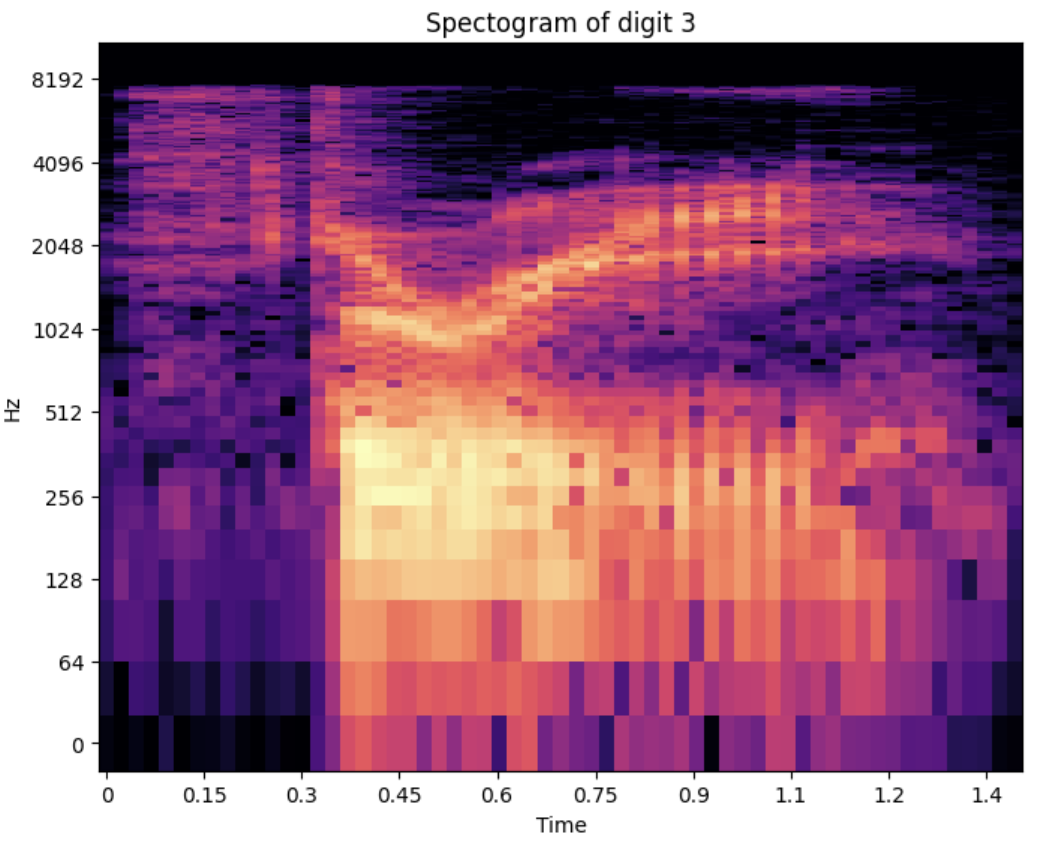
\includegraphics[width=0.6\textwidth]{./graphics/STFT_0.png} % PNG/JPG/PDF
  \caption{Ví dụ về STFT}
  \label{Ví dụ về STFT}
\end{figure}\\



Mặc dù STFT cung cấp thông tin về cả thời gian và tần số, nhưng nó vẫn có hạn chế trong việc cách con người tiếp nhận âm thanh, 
khi tai người cảm nhận tần số phi tuyến (nhạy ở vùng thấp 0-1000Hz, kém nhạy ở vùng cao >1000Hz) và cách để phân biệt các âm sắc khác nhau của 
tai người là tỉ lệ giữa các dải tần.
\subsubsection{Mel-Frequency Cepstral Coefficients (MFCCs):}
Thang Mel: Là thang cao độ cảm nhận, được người nghe đánh giá và có khoảng cách các quãng bằng nhau. 
Điểm tham chiếu giữa thang Mel và phép đo tần số thông thường xác định bằng cách gán cao độ cảm nhận 1000 mels cho âm có tần số 1000~Hz. 
Công thức phổ biến để biến đổi tần số $f$ (Hz) thành $m$ (mels) là:

\begin{equation}
m = 2595 \log_{10} \left( 1 + \frac{f}{700} \right); 
\quad f = 700 \left( 10^{\frac{m}{2595}} - 1 \right)
\end{equation}




\noindent
Để trích xuất \textit{Mel-spectrograms}, ta làm theo các bước như sau:
\begin{itemize}
    \item pre-emphasis: Tăng cường các tần số cao trong tín hiệu âm thanh để cân bằng phổ.
    \item Sử dụng STFT đối với tín hiệu âm thanh.
    \item Biến đổi các biên độ thành dB.
    \item Biến đổi các tần số thành thang Mel.
\end{itemize}

Pre-emphasis là một bộ lọc FIR (Finite Impulse Response) bậc 1, được áp dụng cho mỗi mẫu tín hiệu:

\[
y[n] = x[n] - \alpha x[n-1]
\]

Trong đó:
\begin{itemize}
    \item $x[n]$ là mẫu tín hiệu gốc tại thời điểm $n$,
    \item $y[n]$ là mẫu tín hiệu sau khi áp dụng pre-emphasis,
    \item $\alpha$ là hệ số pre-emphasis, thường lấy giá trị khoảng 0.95 đến 0.97.
\end{itemize}
Mục đích chính của bộ lọc này là để cân bằng phổ (spectral balancing) và tăng cường các tần số cao (boost high frequencies).
\begin{itemize}
    \item Cân bằng Năng lượng Phổ: Tín hiệu giọng nói tự nhiên (đặc biệt là các nguyên âm) có xu hướng có nhiều năng lượng hơn ở các tần số thấp và năng lượng giảm dần ở các tần số cao. Pre-emphasis hoạt động như một bộ lọc thông cao (high-pass filter) để làm phẳng phổ, giúp cho các tần số cao có năng lượng tương đương hơn so với tần số thấp.
    \item Nhấn mạnh Phụ âm: Các thông tin quan trọng để phân biệt âm thanh (như các phụ âm xát: /s/, /f/) thường nằm ở dải tần số cao. Việc tăng cường các tần số này giúp mô hình nhận dạng tập trung vào chúng tốt hơn.
    \item Cải thiện Độ ổn định Số học: Việc cân bằng phổ giúp tránh các vấn đề về độ chính xác số học (numerical precision) trong các bước tính toán FFT sau này, vì năng lượng được phân bổ đều hơn.
\end{itemize}
\noindent
Các bước xây dựng ngân hàng lọc Mel (Mel-filter-banks):
\begin{itemize}
    \item Chọn số lượng dải Mel (n\_mels).
    \item Xây dựng các ngân hàng lọc Mel:
    \begin{itemize}
        \item Biến đổi tần số thấp nhất và cao nhất thành thang Mel.
        \item Tạo các dải Mel cách đều nhau.
        \item Biến đổi các điểm đó trở lại đơn vị Hertz.
        \item Làm tròn đến ngăn tần gần nhất.
        \item Tạo các bộ lọc tam giác.
    \end{itemize}
    \item Áp dụng các ngân hàng lọc Mel đối với quang phổ.
    \begin{equation}
      H_m(k) =
\begin{cases}
0 & \text{for } k < f(m-1) \\
\frac{k - f(m-1)}{f(m) - f(m-1)} & \text{for } f(m-1) \leq k < f(m) \\
\frac{f(m+1) - k}{f(m+1) - f(m)} & \text{for } f(m) \leq k < f(m+1) \\
0 & \text{for } k \geq f(m+1)
\end{cases}
    \end{equation}
    \begin{tabular}{|l|l|}
\hline
\textbf{Tham số} & \textbf{Ý nghĩa} \\
\hline
$H_m(k)$ & Giá trị đầu ra (trọng số) của bộ lọc Mel thứ $m$ tại chỉ số tần số $k$. \\
$m$ & Chỉ số của bộ lọc Mel, với $1 \leq m \leq M$ ($M$ là tổng số bộ lọc). \\
$k$ & Chỉ số bin tần số của kết quả FFT, $0 \leq k < N_{FFT}/2$. \\
$f(m)$ & Chỉ số bin tần số trung tâm (đỉnh tam giác) của bộ lọc thứ $m$. \\
$f(m-1)$ & Chỉ số bin tần số trung tâm của bộ lọc liền kề trước đó. \\
$f(m+1)$ & Chỉ số bin tần số trung tâm của bộ lọc liền kề sau đó. \\
\hline
\end{tabular}\\
\begin{figure}[ht]
  \centering
  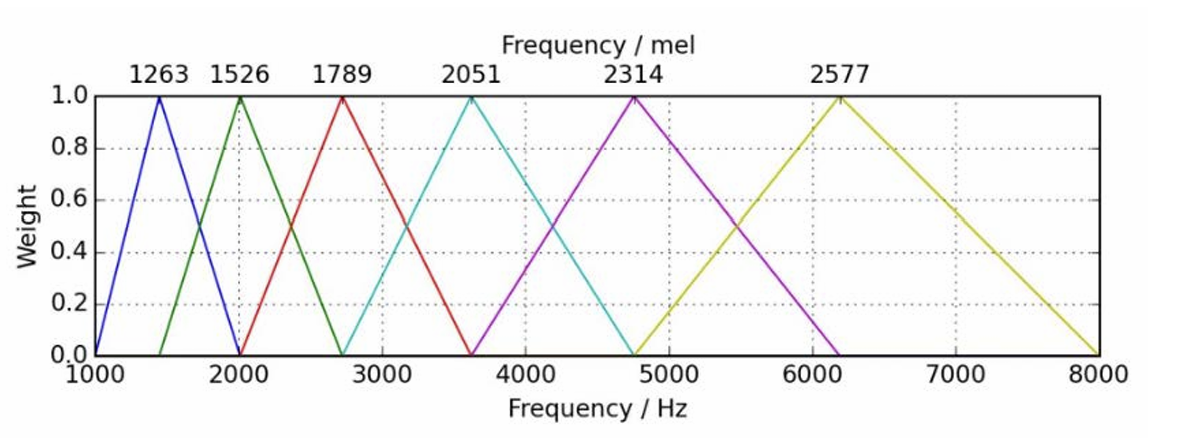
\includegraphics[width=0.5\textwidth]{./graphics/MFCC_0.png} % PNG/JPG/PDF
  \caption{Mel filter banks}
  \label{Mel-filter-banks}
\end{figure}\\
\item Tính năng lượng của dải Mel thứ $m$:
\[
E_m = \sum_{k=0}^{N_{FFT}/2 - 1} |X(k)|^2 \cdot H_m(k)
\]
\item Sau khi có $M$ giá trị năng lượng $E_m$, ta lấy logarit của các giá trị này.
\[
S_m = \ln(E_m)
\]
\item Cuối cùng, áp dụng công thức DCT (loại II) lên $M$ giá trị log-năng lượng $S_m$ để thu được các hệ số MFCC. Công thức tính hệ số MFCC thứ $n$ như sau:
\[
C_n = \sum_{m=1}^{M} S_m \cos\left[ \frac{\pi n (m - 0.5)}{M} \right]
\]
\item Trong đó, ta thường chỉ giữ lại $L$ hệ số đầu tiên (ví dụ $L=13$), nên $n = 0, 1, \ldots, L-1$.
\begin{center}
\begin{tabular}{|l|l|}
\hline
\textbf{Tham số} & \textbf{Ý nghĩa} \\
\hline
$C_n$ & Hệ số MFCC thứ $n$ . \\
$S_m$ & Giá trị Log-năng lượng từ bộ lọc Mel thứ $m$. \\
$M$ & Tổng số lượng bộ lọc Mel (tổng số tam giác). \\
$m$ & Chỉ số của bộ lọc Mel (từ 1 đến $M$). \\
$L$ & Số lượng hệ số MFCC. \\
\hline
\end{tabular}
\end{center}
\end{itemize}

Các hệ số MFCC $C_n$ tính ở bước trước được gọi là hệ số tĩnh (static coefficients). Chúng chỉ mô tả đặc điểm phổ của một khung tín hiệu (frame) tại một thời điểm.

Tuy nhiên, giọng nói là một tín hiệu động (dynamic); cách mà các đặc điểm thay đổi theo thời gian (ví dụ: chuyển tiếp từ phụ âm sang nguyên âm) chứa thông tin nhận dạng cực kỳ quan trọng.

Chúng ta tính toán các hệ số delta (vận tốc) và delta-delta (gia tốc) để nắm bắt thông tin động này.
\\
\begin{figure}[ht]
  \centering
  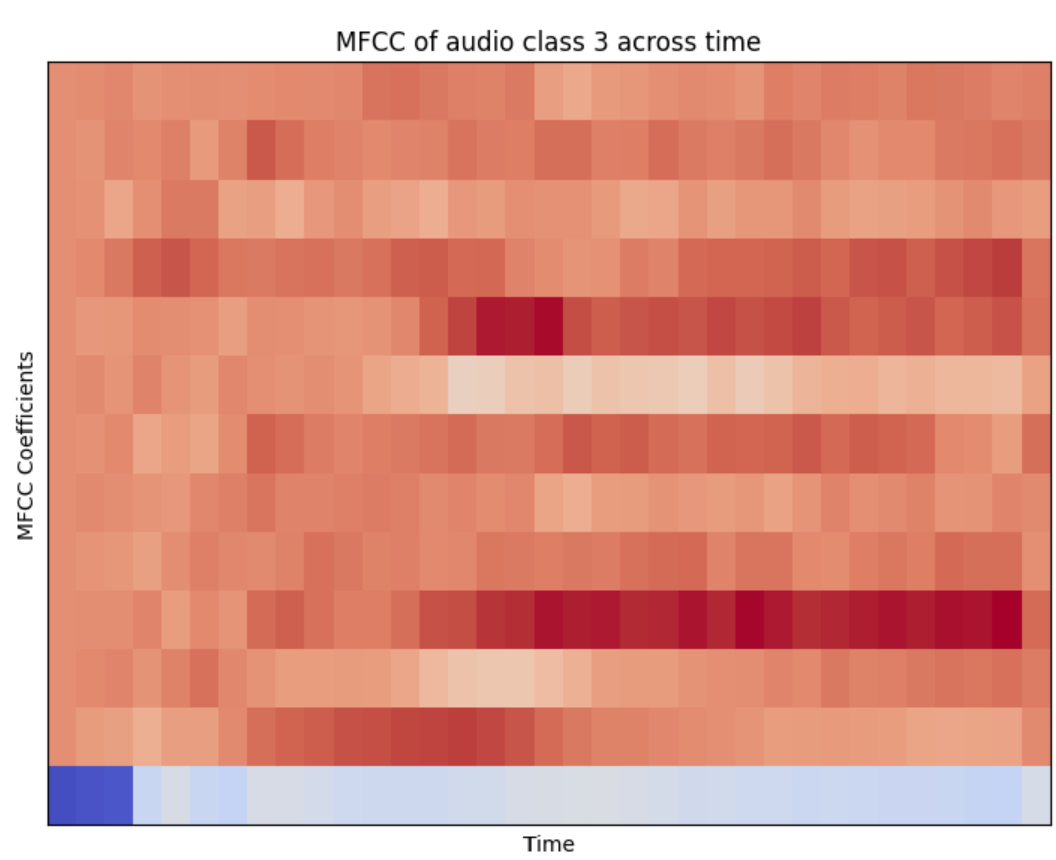
\includegraphics[width=0.6\textwidth]{./graphics/MFCC_1.png} % PNG/JPG/PDF
  \caption{Ví dụ về MFCC, delta và delta-delta}
  \label{Ví dụ về MFCC, delta và delta-delta}
\end{figure}\\



\section{Ứng dụng giải thuật}
\subsection{Tổng quan tập dữ liệu và nhiệm vụ của nhóm:}
Tập dữ liệu được sử dụng trong bài toán này là tập dữ liệu Spoken Digit Dataset, bao gồm các mẫu âm thanh của các chữ số từ 
0 đến 9 được nói bởi nhiều người khác nhau. Mỗi mẫu âm thanh được lưu dưới dạng file WAV. Tập dữ liệu này bao gồm tổng cộng 17000 mẫu, với mỗi chữ số có 1700 mẫu. 
Nguồn dữ liệu: \url{https://www.kaggle.com/datasets/subhajournal/free-spoken-digit-database} \\


Nhiệm vụ của nhóm là xây dựng mười mô hình HMM để nhận diện chính xác chữ số được nói trong mỗi mẫu âm thanh.
\subsection{Thống kê mô tả tập dữ liệu:}
Quan sát sơ bộ tập dữ liệu, ta thấy rằng mỗi lớp âm thanh .